\documentclass{standalone}
\usepackage{tikz,tkz-euclide}
\usepackage{ctex}
\setCJKmainfont{Noto Serif CJK SC}
\usepackage{mhchem,siunitx}
\usetikzlibrary{patterns,patterns.meta,calc}
\usetikzlibrary {decorations.pathmorphing, decorations.pathreplacing, decorations.shapes}
\newcommand{\BottleEmpty}[1][]{
  \begin{scope}[#1]
    \fill[left color=gray,right color=gray,middle color=white](-0.3,2.3)rectangle(0.3,2.7);
    \foreach \x in {-0.5,-0.4,...,0.6}
    {
      \draw[very thin](\x,0.05)circle(0.05);
      \draw[very thin](\x,0.228)circle(0.05);
    }
    \foreach \x in {-0.6,-0.5,...,0.6}
    {
      \draw[very thin](\x+0.05,0.136)circle(0.05);
    }
    \draw[fill=cyan!10!white,fill opacity=0.2](-0.3,2.5)[rounded corners=1pt]--++(0,-0.3)arc(90:180:0.4)[rounded corners=5pt]--(-0.7,0)--(0.7,0)[sharp corners]--(0.7,1.8)[rounded corners=1pt]arc(0:90:0.4)[sharp corners]--++(0,0.3)arc(180:90:0.05)--(-0.35,2.55)arc(90:0:0.05)--cycle;
  \end{scope}
}
\newcommand{\SeparatoryFunnel}[1][]{
  \begin{scope}[#1]
    \draw[ball color=cyan!20!white](0,0.3)circle(0.05);
    \draw[fill=cyan!20!white](-0.05,0.19)rectangle(0.05,0.29);
    \draw[fill=cyan!10!white](-0.1,0.25)rectangle(0.1,0.27);
    \fill[cyan!50!white,fill opacity=0.5](-160:0.2)arc(-160:-20:0.2);
    \draw(110:0.2)arc(110:430:0.2)--++(0,0.05)-|cycle;
    \draw[double distance=1.5pt](0,-0.19)--(0,-1.5);
    \draw(0.75pt,-1.5)--++(0,-0.1)--++(-1.5pt,0.1);
    \draw[thick,gray,line cap=round](-0.07,-0.24)--(0.07,-0.24)(0.07,-0.26)--(0.07,-0.22);
    \fill[cyan!30!lightgray,opacity=0.8](-0.06,-0.28)rectangle(0.06,-0.20);
  \end{scope}
}
\newcommand{\FilledTube}[6][]{
  \begin{scope}[#1,rotate=#2]
    \fill[#4](-#3+#5,0.15)--(0,0.15)arc(-90:0:0.05)--(0.05,-0.2)arc(0:90:0.05)--(-#3+#5,-0.15)--cycle;
    \fill[#6](-#3+#5,-0.15)--(-#3,-0.15)arc(270:90:0.15)--(-#3+#5,0.15)--cycle;
    \draw[fill=cyan!10!white,fill opacity=0.2](-#3,0.15)--(0,0.15)arc(-90:0:0.05)--(0.05,-0.2)arc(0:90:0.05)--(-#3,-0.15)arc(270:90:0.15)--cycle;
  \end{scope}
}

\begin{document}
\small
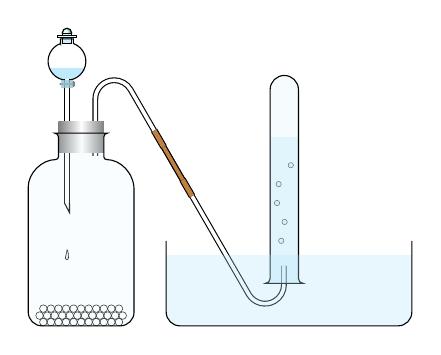
\begin{tikzpicture}[>=stealth,scale=1.2,inner sep=2pt]
  \draw[double distance=1.3pt](0.15,1.8)--(0.15,2.4)arc(180:30:0.2)--++(-60:0.5)coordinate(a)--++(-60:2.0)arc(-150:0:0.2)--++(0,0.2);
  \draw[double distance=1.7pt,double=brown](a)--++(-60:0.2)([shift=(-60:0.6)]a)--++(-60:0.2);
  \draw[double distance=1.3pt,double=brown]([shift=(-60:0.2)]a)--++(-60:0.4);
  \SeparatoryFunnel[xshift=-0.15cm,yshift=2.8cm]
  \draw[very thin,fill=cyan!20!white](-0.15,0.8)to[out=-90,in=180]+(0,-0.1)to[out=0,in=90]cycle;
  \BottleEmpty[scale=0.8]
  \foreach \y in {0.9,1.1,1.3,1.5,1.7}
  {
    \draw[very thin,fill=lightgray!20](2.15+0.1*rand,\y)circle(0.8pt);
  }
  \FilledTube[xshift=2.15cm,yshift=0.5cm]{-90}{2.0}{cyan!30!white,fill opacity=0.4}{0.5}{cyan!10!white,fill opacity=0.2}
  \fill[cyan!30!white,fill opacity=0.3,rounded corners=5pt](0.9,0.75)|-(3.5,0)--(3.5,0.75);
  \draw[rounded corners=5pt](0.9,0.9)|-(3.5,0)--(3.5,0.9);
\end{tikzpicture}
\end{document}